\documentclass[11pt]{article}
\usepackage[utf8]{inputenc}
%\geometry{showframe}% for debugging purposes -- displays the margins

\newcommand{\E}{\mbox{E}}
\newcommand{\MSE}{\mbox{MSE}}
\newcommand{\var}{\mbox{var}}
\newcommand{\by}{\textbf{y}}

%% ys
\usepackage[shortlabels]{enumitem}
\usepackage{geometry}
\usepackage{bm}
\usepackage{amssymb}
\usepackage{algorithm}
\usepackage{algpseudocode}
\usepackage{xcolor}
\usepackage{listings}
\geometry{a4paper,scale=0.75}
\newcommand{\jie}{$\star$ }
\newcommand{\bx}{\bm{x}}
\newcommand{\iid}{\overset{\text{iid}}{\sim}}
\newcommand{\half}{\frac{1}{2}}
\newcommand{\ynote}[1]{\color{red} #1 \color{black}}
%% ys

\usepackage{amsmath,amssymb,amsfonts,amsthm} % amsmath package, useful for mathematical formulas
%\usepackage[garamond]{mathdesign}
\usepackage{hyperref}
\hypersetup{colorlinks}% uncomment this line if you prefer colored hyperlinks (e.g., for onscreen viewing)


\newtheorem{theorem}{Theorem}
\newtheorem{lemma}[theorem]{Lemma}

% Set up the images/graphics package
\usepackage{graphicx}
\setkeys{Gin}{width=\linewidth,totalheight=\textheight,keepaspectratio}
\graphicspath{{graphics/}}

\title{Exercises 3 $\cdot$ SDS 383D \\ Exercises 3: Bayes and the Gaussian linear model}
%\author[ ]{ }
\date{}  % if the \date{} command is left out, the current date will be used

% The following package makes prettier tables.  We're all about the bling!
\usepackage{booktabs}

% The units package provides nice, non-stacked fractions and better spacing
% for units.
\usepackage{units}

% The fancyvrb package lets us customize the formatting of verbatim
% environments.  We use a slightly smaller font.
\usepackage{fancyvrb}
\fvset{fontsize=\normalsize}

% Small sections of multiple columns
\usepackage{multicol}

% Provides paragraphs of dummy text
\usepackage{lipsum}

% These commands are used to pretty-print LaTeX commands
\newcommand{\doccmd}[1]{\texttt{\textbackslash#1}}% command name -- adds backslash automatically
\newcommand{\docopt}[1]{\ensuremath{\langle}\textrm{\textit{#1}}\ensuremath{\rangle}}% optional command argument
\newcommand{\docarg}[1]{\textrm{\textit{#1}}}% (required) command argument
\newenvironment{docspec}{\begin{quote}\noindent}{\end{quote}}% command specification environment
\newcommand{\docenv}[1]{\textsf{#1}}% environment name
\newcommand{\docpkg}[1]{\texttt{#1}}% package name
\newcommand{\doccls}[1]{\texttt{#1}}% document class name
\newcommand{\docclsopt}[1]{\texttt{#1}}% document class option name

\newcommand{\N}{\mbox{N}}
\newcommand{\thetahat}{\hat{\theta}}
\newcommand{\sigmahat}{\hat{\sigma}}
\newcommand{\betahat}{\hat{\beta}}


\begin{document}

\maketitle% this prints the handout title, author, and date


\section{A simple Gaussian location model}

Take a simple Gaussian model with unknown mean and variance:
\begin{equation}
\label{eqn:normal_model}
(y_i \mid \theta, \sigma^2) \sim N(\theta, \sigma^2) \; , \quad i = 1, \ldots, n \, .
\end{equation}
Let $\bf{y}$ be the vector of observations $\textbf{y} = (y_1, \ldots, y_n)^T$.

Suppose we place conjugate normal and inverse-gamma priors on $\theta$ and $\sigma^2$, respectively:
\begin{align*}
(\theta \mid \sigma^2) &\sim N(\mu, \tau^2 \sigma^2) \\
\sigma^2 &\sim \mbox{Inv-Gamma}\left( \frac{d}{2}, \frac{ \eta}{2} \right) \, ,
\end{align*}
where $\mu$, $\tau > 0$, $d>0$ and $\eta > 0$ are fixed scalar hyperparameters.  Note a crucial choice here: the error variance appears in the prior for $\theta$.  This affects the interpretation of the hyperparameter $\tau$, which is not the prior variance of $\theta$, but rather the prior signal-to-noise ratio.  This is pretty common thing to do in setting up priors for location parameters: to scale the prior by the error variance.  There are a few good reasons to do this, but historically the primary one has been analytical convenience (as you'll now see).

Here's a sensible way to interpret each of these four parameters:
\begin{itemize}
\item $\mu$ is a prior guess for $\theta$.
\item $\tau$ is a prior signal-to-noise ratio---that is, how disperse your prior is for $\theta$, relative to the error standard deviation $\sigma$.
\item $d$ is like a ``prior sample size'' for the error variance $\sigma^2$.
\item $\eta$ is like a ``prior sum of squares'' for the error variance $\sigma^2$.  More transparently, $\eta/d$ is like a prior guess for the error variance $\sigma^2$.  It's not exactly the prior mean for $\sigma^2$, but it's close to the prior mean as $d$ gets larger, since the inverse-gamma(a,b) prior has expected value
$$
E(\sigma^2) = b/(a-1) =  \frac{\eta / 2}{d/2 - 1} = \frac{\eta}{d - 2} \approx \eta/d
$$
if $d$ is large.\footnote{This expression is only valid if $d > 2$.}
\end{itemize}

What is meant by the phrases ``prior sample size'' and ``prior sum of squares''?  Well, remember that conjugate priors always resemble the likelihood functions that they're intended to play nicely with.  The two relevant quantities in the likelihood function for $\sigma^2$ are the sample size and the sums of squares.  The prior here is designed to mimic the likelihood function for $\sigma^2$ that you'd get if you hallucinated a previous data set with sample size $d$ and sums of squares $\eta$.

\paragraph{Precisions are easier than variances.}  It's perfectly fine to work with this form of the prior, and it's easier to interpret this way.  But it turns out that we can make the algebra a bit cleaner by working with the precisions $\omega = 1/\sigma^2$ and $\kappa = 1/\tau^2$ instead.
\begin{align*}
(\theta \mid \omega) &\sim N(\mu, (\omega \kappa)^{-1}) \\
\omega &\sim \mbox{Gamma}\left( \frac{d}{2}, \frac{ \eta}{2} \right) \, .
\end{align*}

This means that the joint prior for $(\theta, \omega)$ has the form
\begin{equation}
\label{eqn:normal_gamma_prior1}
p(\theta, \omega) \propto \omega^{(d+1)/{2} - 1} \exp \left\{ - \omega \cdot \frac{\kappa (\theta - \mu)^2}{2}  \right\}
\cdot \exp\left\{ -  \omega \cdot \frac{\eta}{2}  \right\} 
\end{equation}
This is often called the \textit{normal/gamma} prior for $(\theta, \omega)$ with parameters $(\mu, \kappa, d, \eta)$, and it's equivalent to a normal/inverse-gamma prior for $(\theta, \sigma^2)$.  (The interpretation of $\kappa$ is like a prior sample size for the mean $\theta$.)  Note: you can obviously write this joint density in Equation \ref{eqn:normal_gamma_prior1} in a way that combines the exponential terms, but this way keeps the bit involving $\theta$ separate, so that you can recognize the normal kernel.\footnote{The term ``kernel'' is heavily overloaded in statistics. \href{http://en.wikipedia.org/wiki/Kernel_(statistics)\#In_Bayesian_statistics}{See Wikipedia for the sense in which I mean the term.}  }


\begin{enumerate}[(A)]


\item By construction, we know that the marginal prior distribution $p(\theta)$ is a gamma mixture of normals.  Show that this takes the form of a centered, scaled $t$ distribution: 
$$
p(\theta) \propto \left(1+ \frac{1}{\nu} \cdot \frac{(x - m)^2}{s^2}  \right)^{-\frac{\nu+1}{2}}
$$
with center $m$,  scale $s$, and degrees of freedom $\nu$, where you fill in the blank for $m$, $s^2$, and $\nu$ in terms of the four parameters of the normal-gamma family.  Note: you did a problem just like this on a previous exercise!  This shouldn't be a lengthy re-derivation.

\bigskip
\jie
$$\theta|w \sim N(m,(w\kappa)^{-1}),$$
$$w \sim Ga(\frac{d}{2}, \frac{\eta}{2}).$$
The marginal distribution of $\theta$ is
\begin{align*}
    p(\theta) &= \int p(\theta|w) p(w) dw \\
    &\propto \int \omega^{(d+1)/{2} - 1} \exp \left\{ - \omega \cdot \frac{\kappa (\theta - \mu)^2}{2}  \right\} \cdot \exp\left\{ -  \omega \cdot \frac{\eta}{2}  \right\} d\omega\\
    &\propto \int \omega^{(d+1)/{2} - 1} \exp \left\{ - \omega \cdot (\frac{\eta}{2} + \frac{\kappa (\theta - \mu)^2}{2} ) \right\} d\omega \\
    &\propto \int \frac{(\frac{\eta}{2} + \frac{\kappa (\theta - \mu)^2}{2} )^{\frac{d+1}{2}} }{\Gamma(\frac{d+1}{2})} w^{\frac{d+1}{2} -1} \exp \{- \omega \cdot (\frac{\eta}{2} + \frac{\kappa (\theta - \mu)^2}{2} ) \} dw \cdot \frac{\Gamma(\frac{d+1}{2})}{(\frac{\eta}{2} + \frac{\kappa (\theta - \mu)^2}{2} )^{\frac{d+1}{2}} } \\
    &\propto [\eta+\kappa (\theta - \mu)^2]^{-\frac{d+1}{2}} \\
    &\propto [1+\frac{1}{d}(\theta-\mu)^2/(\frac{\eta}{\kappa d})]^{-\frac{d+1}{2}} \\
    &\equiv t(d,\mu,(\frac{\eta}{\kappa d})^{1/2}).
\end{align*}

\item Assume the normal sampling model in Equation \ref{eqn:normal_model} and the normal-gamma prior in Equation \ref{eqn:normal_gamma_prior1}.  Calculate the joint posterior density $p(\theta, \omega \mid \textbf{y})$, up to constant factors not depending on $\omega$ or $\theta$.  Show that this is also a normal/gamma prior in the same form as above:
\begin{equation}
\label{eqn:normal_gamma_post}
p(\theta, \omega \mid \by) \propto \omega^{(d^\star+1)/2 - 1} \exp \left\{ - \omega \cdot \frac{\kappa^\star (\theta - \mu^\star)^2}{2}  \right\}
\cdot \exp\left\{ -  \omega \cdot \frac{\eta^\star}{2}  \right\} 
\end{equation}
From this form of the posterior, you should able to read off the new updated parameters, by pattern-matching against the functional form in Equation \ref{eqn:normal_gamma_prior1}:
\begin{itemize}
\item $\mu \longrightarrow \mu^\star =  \; ?$
\item $\kappa \longrightarrow \kappa^\star =  \; ?$
\item $d \longrightarrow d^{\star} =  \; ?$
\item $\eta \longrightarrow \eta^\star = \; ?$
\end{itemize}
You may notice that my parameterization of the normal-gamma in Equation \ref{eqn:normal_gamma_prior1} differs from, say, the one you might find in textbooks or on websites.  I've chosen this parameterization in order to make these four updates for the parameters, above, as simple-looking and intuitive as possible.


Tip: this one is a bit of an algebra slog, with a lot of completing the square, collecting common terms, and cancelling positives with negatives.  For example, to make the calculations go more easily, you might first show (or recall, from a previous exercise) that the likelihood can be written in the form
$$
p(\by \mid \theta, \omega) \propto \omega^{n/2} \exp \left\{ - \omega \cdot \left( \frac{S_y + n(\bar{y} - \theta)^2}{2} \right) \right\} \, ,
$$
where $S_y = \sum_{i=1}^n (y_i - \bar{y})^2$ is the sum of squares for the $\by$ vector.  This expresses the likelihood in terms of the two statistics $\bar{y}$ and $S_y$, which you may recall from your math-stat course are sufficient statistics for $(\theta, \sigma^2)$.

Take care in ignoring constants here: some term that is constant in $\theta$ may not be constant in $\omega$, and vice versa.  You're focusing on the joint posterior, so you can't ignore anything that has a $\theta$ or $\omega$ in it.

\bigskip
\jie
\begin{align*}
    p(\theta,\omega|y) &\propto p(y|\theta,\omega) p(\theta,\omega) \\
    &\propto (\omega)^{\frac{n}{2}} \exp\left\{ -\frac{\omega}{2} \sum_i [S_y + n(\theta - \bar{y})^2] \right\} \cdot \omega^{\frac{d+1}{2}-1} \exp \left\{ -\omega \frac{\kappa (\theta-\mu)^2}{2} \right\} \cdot \exp \left\{ -\omega \frac{\eta}{2} \right\} \\
    & = \omega^{\frac{d+n+1}{2}-1} \exp\left\{ -\frac{\omega}{2} [n\theta^2 - 2n \bar{y}\theta + n\bar{y}^2 + \kappa \theta^2 - 2\kappa \mu \theta + \kappa \mu^2 + \eta + S_y] \right\} \\
    & = \omega^{\frac{d+n+1}{2}-1} \exp\left\{ -\frac{\omega}{2} [(n+\kappa)(\theta - \frac{n\bar{y} + \kappa \mu}{n+\kappa})^2 - \frac{(n\bar{y} + \kappa \mu)^2}{n+\kappa} + \eta + S_y +n\bar{y}^2 + \kappa \mu^2] \right\}
\end{align*}
Therefore,
\begin{itemize}
\item $\mu \longrightarrow \mu^\star =  \frac{n\bar{y} + \kappa \mu}{n+\kappa}$
\item $\kappa \longrightarrow \kappa^\star = n + \kappa$
\item $d \longrightarrow d^{\star} =  d+n$
\item $\eta \longrightarrow \eta^\star = \eta + S_y +n\bar{y}^2 + \kappa \mu^2 - \frac{(n\bar{y} + \kappa \mu)^2}{n+\kappa} = \eta +\sum_i y_i^2 + \kappa \mu^2 - \frac{(n\bar{y} + \kappa \mu)^2}{n+\kappa}$
\end{itemize}

\item From the joint posterior you just derived, what is the conditional posterior distribution $p(\theta \mid \by, \omega)$?  Note: this should require no calculation---you should just be able to read it off directly from the joint distribution, since you took care to set up things so that the joint posterior was in the same form as Equation \ref{eqn:normal_gamma_prior1}.

\bigskip
\jie
$$p(\theta|\omega,y) = N(\mu^*, (\omega\kappa^*)^{-1}) = N(\frac{n\bar{y} + \kappa \mu}{n+\kappa}, (\omega(n + \kappa))^{-1})$$
\bigskip

\item From the joint posterior you calculated in (A), what is the marginal posterior distribution $p(\omega \mid \by)$?  Unlike the previous question, this one doesn't come 100\% for free---you have to integrate over $\theta$.  But it shouldn't be too hard, since you can ignore constants not depending on $\omega$ in calculating this integral.

\bigskip
\jie
$$p(\theta, \omega \mid \by) \propto \omega^{(d^\star+1)/2 - 1} \exp \left\{ - \omega \cdot \frac{\kappa^\star (\theta - \mu^\star)^2}{2}  \right\}
\cdot \exp\left\{ -  \omega \cdot \frac{\eta^\star}{2}  \right\} $$
Then,
\begin{align*}
    p(\omega \mid \by) &\propto \int \omega^{(d^\star+1)/2 - 1} \exp \left\{ - \omega \cdot \frac{\kappa^\star (\theta - \mu^\star)^2}{2}  \right\}
\cdot \exp\left\{ -  \omega \cdot \frac{\eta^\star}{2}  \right\} d\theta \\
&= \omega^{(d^\star+1)/2 - 1} \cdot \exp\left\{ -  \omega \cdot \frac{\eta^\star}{2}  \right\} \int \exp \left\{ - \omega \cdot \frac{\kappa^\star (\theta - \mu^\star)^2}{2}  \right\} d\theta \\
&\propto \omega^{(d^\star+1)/2 - 1} \cdot \exp\left\{ -  \omega \cdot \frac{\eta^\star}{2}  \right\} (\kappa^* \omega)^{-\half} \\
&\propto \omega^{d^\star/2 - 1}\cdot \exp\left\{ -  \omega \cdot \frac{\eta^\star}{2}  \right\} \\
&= Gamma(\frac{d^\star}{2},\frac{\eta^\star}{2})
\end{align*}

\bigskip

\item Show that the marginal posterior $p(\theta \mid \by)$ takes the form of a centered, scaled $t$ distribution and express the parameters of this $t$ distribution in terms of the four parameters of the normal-gamma posterior for $(\theta, \omega)$.  Note: since you've set up the normal-gamma family in this careful conjugate form, this should require no extra work.  It's just part (A), except for the posterior rather than the prior.
$$ p(\theta|y) = t(d^*,\mu^*,(\frac{\eta^*}{\kappa^* d^*})^{1/2})$$

\item True or false: in the limit as the prior parameters $\kappa$, $d$, and $\eta$ approach zero, the priors $p(\theta)$ and $p(\omega)$ are valid probability distributions.  (Remember that a valid probability distribution must integrate to 1 (or something finite, so that it can normalized to integrate to 1) over its domain.)

\bigskip
\jie FALSE. Because we know the marginal prior of $\theta$, t distribution, is undefined.

\item True or false: in the limit as the prior parameters $\kappa$, $d$, and $\eta$ approach zero, the posteriors $p(\theta \mid \by)$ and $p(\omega \mid \by)$ are valid probability distributions.

\bigskip
\jie TRUE. We call tell from the result in (C) that when the hyper parameters go to 0, the conditional posteriors are well defined.

\item Your result in (E) implies that a Bayesian credible interval for $\theta$ takes the form
$$
\theta \in m \pm t^{\star} \cdot s \, ,
$$
where $m$ and $s$ are the posterior center and scale parameters from (E), and $t^\star$ is the appropriate critical value of the t distribution for your coverage level and degrees of freedom (e.g.~it would be 1.96 for a 95\% interval under the normal distribution).

True or false: In the limit as the prior parameters $\kappa$, $d$, and $\eta$ approach zero, the Bayesian credible interval for $\theta$ becomes identical to the classical (frequentist) confidence interval for $\theta$ at the same confidence level.

$$
\theta \in \mu^* \pm t^{\star} \cdot (\frac{\eta^*}{\kappa^* d^*})^{1/2} \, ,
$$

\begin{itemize}
\item $\mu^\star =  \frac{n\bar{y} + \kappa \mu}{n+\kappa} \rightarrow \bar{y}$
\item $\kappa^\star = n + \kappa \rightarrow n $
\item $d^{\star} =  d+n \rightarrow n$
\item $\eta^\star = \eta + S_y +n\bar{y}^2 + \kappa \mu^2 - \frac{(n\bar{y} + \kappa \mu)^2}{n+\kappa} = \eta +\sum_i y_i^2 - \frac{(n\bar{y} + \kappa \mu)^2}{n+\kappa} \rightarrow S_y$
\end{itemize}

$$
\theta \in \bar{y} \pm t^{\star} \cdot \frac{\sqrt{S_y}}{n} \, ,
$$
The frequentist confidence interval
$$\theta \in \bar{y} \pm t^{\star} \cdot \frac{\sqrt{\frac{1}{n-1}S_y}}{\sqrt{n}}.$$
Identical? (Almost).

\end{enumerate}


\newpage 

\section{The conjugate Gaussian linear model}

Now consider the homoskedastic Gaussian linear model
$$
(\by \mid \beta, \sigma^2) \sim \N(X\beta, (\omega \Lambda)^{-1} ) \, ,
$$
where $\by$ is an $n$ vector of responses, $X$ is an $n \times p$ matrix of features, and $\omega = 1/\sigma^2$ is the error precision, and $\Lambda$ is some known matrix.  A typical setup would be $\Lambda = I$, the $n \times n$ identity matrix, so that the residuals of the model are i.i.d.~normal with variance $\sigma^2$ (hence homoskedastic).  But we'll want to consider other setups as well, so we'll leave a generic $\Lambda$ matrix in the sampling model for now.

Note that when we write the model this way, we typically assume one of two things: either (1) that both the $y$ variable and all the $X$ variables have been centered to have mean zero, so that an intercept is unnecessary; or (2) that $X$ has a vector of 1's as its first column, so that the first entry in $\beta$ is actually the intercept.

We'll again work in terms of the precision $\omega = \sigma^2$, and consider a normal--gamma prior for $\beta$:
\begin{align}
(\beta \mid \omega) &\sim N(m, (\omega K)^{-1}) \\
\omega &\sim \mbox{Gamma}(d/2, \eta/2) \, .
\end{align}
Here $K$ is a $p \times p$ precision matrix in the multivariate normal prior for $\beta$, which we assume to be known.

The items below follow a parallel path to the derivations you did for the Gaussian location model, except for the multivariate case.  Don't reinvent the wheel if you don't have to: you should be relying heavily on your previous results about the multivariate normal distribution.\footnote{That is, if you find yourself completing the square over and over again with matrices and vectors, you should stop and revisit your Exercises 1 solutions.}

\subsection{Basics}

\begin{enumerate}[(A)]

\item Derive the conditional posterior $p(\beta \mid \by, \omega)$.

\begin{align*}
    p(\beta,w \mid y) &\propto w^{\frac{n}{2}} |\Lambda|^{\half} \exp\{-\frac{w}{2}(y-X\beta)^T\Lambda(y-X\beta) \} \\& \cdot w^{\frac{p}{2}} |K|^{\half} \exp\{-\frac{w}{2} (\beta - m)^T K(\beta-m) \} \cdot w^{\frac{d}{2}-1} \exp\{-\frac{\eta}{2}w\}
\end{align*}
\begin{align*}
    p(\beta \mid y,w) &\propto \exp \{-\frac{w}{2} [\beta^TX^T\Lambda X \beta - 2\beta^T X^T \Lambda y + \beta^T K \beta - \beta^T K m]\} \\
    &\propto \exp \{-\frac{w}{2} [\beta^T (X^T\Lambda X + K) \beta - 2\beta^T(X^T \Lambda y + K m)]\} \\
    &= N(\mu_\beta, w^{-1}V_\beta),
\end{align*}
where $V_\beta = (X^T \Lambda X + K)^{-1}$, $\mu_\beta = V_\beta (X^T \Lambda y + Km)$.

\item Derive the marginal posterior $p(\omega \mid \by)$.

\begin{align*}
    p(w \mid y) &\propto w^{\frac{n+p+d}{2} -1} \exp\{-\frac{\eta}{2}w\} \cdot \exp\{-\frac{w}{2}[y^T\Gamma y + m^T K m]\} \\&\cdot \int \exp \{ -\frac{w}{2} [\beta^TX^T\Lambda X \beta - 2\beta^T X^T \Lambda y + \beta^T K \beta - \beta^T K m]  \} d\beta \\
    &\propto w^{\frac{n+p+d}{2} -1} \exp\{-\frac{\eta}{2}w\} \cdot \exp\{-\frac{w}{2}[y^T\Gamma y + m^T K m]\} \cdot w^{-\frac{p}{2}} \exp\{\frac{w}{2} \mu_\beta^T V_\beta^{-1} \mu_\beta \} \\
    &\propto w^{\frac{n}{2}+\frac{d}{2} -1} \exp\{ -w \half[\eta + y^T\Gamma y + m^T K m - \mu_\beta^T V_\beta^{-1} \mu_\beta ] \} \\
    &= Ga(\frac{d_w}{2}, \frac{\eta_w}{2}),
\end{align*}
where $d_w = n+ d$, $\eta_w = \eta + y^T\Lambda y + m^T K m - \mu_\beta^T V_\beta^{-1} \mu_\beta $.

\item Putting these together, derive the marginal posterior $p(\beta \mid \by)$.

\begin{align*}
    p(\beta \mid y) &\propto \int p(\beta \mid w,y) p(w \mid y) dw \\
    &\propto \int w^{\frac{p}{2}} |V_\beta|^{\half} \exp\{-\frac{w}{2} (\beta-\mu_\beta)^T V_\beta^{-1} (\beta-\mu_\beta) \} \cdot w^{\frac{d_w}{2}-1} \exp\{-w\frac{\eta_w}{2}\} dw \\
    & \propto \int w^{\frac{p}{2}+\frac{d_w}{2} - 1} \exp\{-w \half[\eta_w + (\beta-\mu_\beta)^T V_\beta^{-1} (\beta-\mu_\beta)]\} dw \\
    &= \frac{\Gamma(\frac{p}{2} + \frac{d_w}{2})}{\{\half[\eta_w + (\beta-\mu_\beta)^T V_\beta^{-1} (\beta-\mu_\beta)] \}^{\frac{p}{2} + \frac{d_w}{2}}} \\
    &\propto [\eta_w + (\beta-\mu_\beta)^T V_\beta^{-1} (\beta-\mu_\beta)] \}^{-\frac{(p+d_w)}{2}} \\
    &\propto [1 + \frac{1}{d_w}(\beta-\mu_\beta)^T ((\frac{\eta_w}{d_w})V_\beta)^{-1} (\beta-\mu_\beta)] \}^{-\frac{(p+d_w)}{2}} \\
    &= t(df=d_w, \mu_\beta, (\frac{\eta_w}{d_w})V_\beta )
\end{align*}

\end{enumerate}

\subsection{Example}

 Take a look at the data in ``greenbuildings.csv'' from the class website, and consider the following short case study in regression.  In commercial real estate, issues of eco-friendliness are intimately tied up with ordinary decisions about how to allocate capital.   Every new project involves negotiating a trade-off between costs incurred and benefits realized over the lifetime of the building. In this context, the decision to invest in eco-friendly buildings could pay off in many possible ways.  Of course, at the end of the day, tenants may or may not be willing to pay a premium for rental space in green buildings.  We can only find out by carefully examining data on the commercial real-estate market.

The file ``greenbuildings.csv''  contains data on over 7,000 commercial rental properties from across the United States.  Of these, 685 properties have been awarded either LEED or EnergyStar certification as a green building.  The basic idea is that a commercial property can receive a green certification if its energy efficiency, carbon footprint, site selection, and building materials meet certain environmental benchmarks.  A group of real estate economists constructed the data set in the following way.  They first sampled 679 green-certified buildings listed on the LEED or EnergyStar websites, and cross-referenced those buildings with data from the CoStar Group (\url{www.costar.com}), a standard data vendor in commercial real estate.  In order to provide a control population, each of these 685 buildings was matched to a cluster of nearby commercial buildings in the CoStar database.  Each small cluster contains one green-certified building, and all non-rated buildings within a quarter-mile radius of the certified building.  On average, each of the 679 clusters contains roughly 12 buildings.

For our purposes, the variables we'll use are:
\begin{enumerate}
\item Rent: rent in dollars per square foot per year (the standard measure in commercial real estate)  
\item leasing rate: what percentage (0-100 scale) of the building is actually leased to a tenant
\item green rating: 0/1, whether the building has a green certification  
\item CityMarketRent: an index of commercial real estate prices for the market in which the building is located  
\item age: age of the building in years
\item class a, class b: indicators for whether the building is class A or class B (if both are 0, the building is class C)  
\end{enumerate}

To build a model here, first define a new response variable, revenue per square foot, defined as the Rent divided by the leasing rate, times 100.  This represents how much actual revenue the property brings in per square foot.  This will be your response variable.  As predictors, using green rating, City Market Rent, age, class a, and class b (and an intercept, of course).  Fit the (homoskedastic) Bayesian linear model to this data set, choosing $\Lambda = I$ and something diagonal and pretty vague for the prior precision matrix $K = \mbox{diag}(\kappa_1, \kappa_2)$.

What is a 95\% Bayesian credible interval for the coefficient on the green rating variable?  How does your result compare to the classical 95\% confidence interval, e.g. from lm in R?  What does a histogram of the model residuals reveal?  (Here you can define the residual vector as $y - X \hat{\beta}$, where $\hat{\beta}$ is the posterior mean.)  Are you happy with your model?  Why or why not?  

\bigskip
\jie
The credible interval for coefficient on the green rating variable
$$(\hat{\beta}_2 - t_{d_w,0.025}\hat{\sigma}_\beta,\hat{\beta}_2 + t_{d_w,0.025}\hat{\sigma}_\beta).$$
The Bayesian credible interval is $( 0.5451348 , 2.299273 )$, and the confidence interval from the lm() function is $(0.5447429, 2.299667)$, which are almost the same.

Figure \ref{fig:hist_res} shows the histogram of the model residual.
\begin{figure}[h]
    \centering
    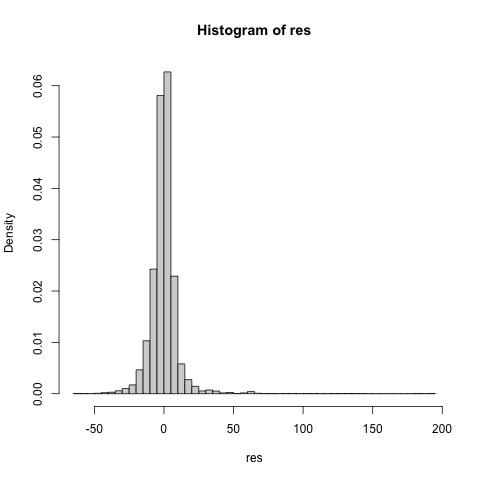
\includegraphics[width=0.6\textwidth]{Ex3/figures/res.jpeg}
    \caption{The histogram of the model residual.}
    \label{fig:hist_res}
\end{figure}

However, under this model the some of the errors of the estimates are large, which is not desirable. And the assumption of the homogeneous variance might not be true. Additionally, from the plot we can tell that the normal assumption is not the best choice of the dataset.  

\subsection{A heavy-tailed error model}


Now it's time for your first ``real'' use of the hierarchical modeling formalism to do something cool.  Here's the full model you'll be working with:
\begin{align}
(\by \mid \beta, \omega, \Lambda) &\sim N(X \beta, (\omega \Lambda)^{-1}) \\
\Lambda &= \mbox{diag}(\lambda_1, \ldots, \lambda_n) \\
\lambda_i &\stackrel{iid}{\sim} \mbox{Gamma}(h/2, h/2) \\
(\beta \mid \omega) &\sim N(m, (\omega K)^{-1}) \\
\omega &\sim \mbox{Gamma}(d/2, \eta/2) \, .
\end{align}
where $h$ is a fixed hyperparameter.

\begin{enumerate}[(A)]


\item Under this model, what is the implied conditional distribution $p(y_i \mid X, \beta, \omega)$?  Notice that $\lambda_i$ has been marginalized out.  This should look familiar.

\item What is the conditional posterior distribution $p(\lambda_i \mid \by, \beta, \omega)$?

\item Combining these results with those from the ``Basics'' subsection above, code up a \href{http://en.wikipedia.org/wiki/Gibbs_sampling}{Gibbs sampler} that repeatedly cycles through sampling the following three sets of conditional distributions.
\begin{itemize}
\item $p(\beta \mid \by, \omega, \Lambda)$
\item $p(\omega \mid \by, \Lambda)$
\item $p(\lambda_i \mid \by, \beta, \omega)$
\end{itemize}
The first two should follow identically from your previous results, except that we are explicitly conditioning on $\Lambda$, which is now a random variable rather than a fixed hyperparameter.  If you cycle through these conditional posterior draws a few thousand times, you will build up a Markov-chain Monte Carlo (MCMC) sample from the joint posterior distribution $p(\beta, \omega, \Lambda \mid \by)$.  Why this technique works for getting posterior draws is the subject of a different course, but hopefully it is reasonably intuitive.

Now use your Gibbs sampler (with at least a few thousand draws) to fit this model to the green buildings data for an appropriate choice of $h$.  Are you happier with the fit?  What's going on here (i.e.~what makes the model more or less appropriate for the data)?\footnote{An interesting plot will be a plot of the posterior mean of $1/\lambda_i$ for each data point.}  How does the 95\% credible interval on each model term compare with the credible intervals you got under the homoskedastic linear model in the previous section?  Are there certain regions of predictor space that seem to be associated with higher variance residuals?  

\end{enumerate}


\end{document}



